\problema{7}{Difusión 1D transitoria con Crank--Nicolson}{7}

\begin{enunciado}
Considere $\dfrac{1}{v}\dfrac{\partial\varphi}{\partial t} = D\varphi_{xx} - \Sigma_a\varphi$ con
$\varphi = 0$ en ambas fronteras. Tome $v = 1$, $D/h^2 = 1$, $\Sigma_a = 0$ y tres nodos interiores,
de modo que $\dfrac{\dd\vect{\varphi}}{\dd t} = -\mat{A}\vect{\varphi}$, $\mat{A} = \tridiag(-1, 2, -1)$.
\begin{enumerate}[label=(\alph*)]
  \item Escriba el esquema CN en forma matricial.
  \item Con $\Delta t = \tfrac12$ y $\vect{\varphi}^0 = (0, 1, 0)^T$, calcule $\vect{\varphi}^1$
        resolviendo con la factorización triple.
  \item Los valores propios de $\mat{A}$ son $2 - \sqrt2$, $2$, $2 + \sqrt2$. Obtenga el factor de
        amplificación de cada modo en CN y pruebe que $|R_j| < 1$ para todo $\Delta t > 0$.
  \item Muestre que Euler explícito requiere $\Delta t < 2/\rho(\mat{A})$ y que con $\Delta t = 1$ es
        inestable, mientras que CN es estable. ¿Qué comportamiento presenta el modo de mayor
        frecuencia en CN con $\Delta t = 1$?
\end{enumerate}
\end{enunciado}

% ---------------------------------------------------------------------
\subsubsection*{Solución}
% ---------------------------------------------------------------------

Primero se multiplica la ecuacion por $v$ para dejar sola la derivada en el tiempo:
\[
  \frac{1}{v}\frac{\partial\varphi}{\partial t} = D\varphi_{xx} - \Sigma_a\varphi
  \quad
  \quad
  \quad
  \quad
  \frac{\partial\varphi}{\partial t} = vD\,\frac{\partial^2\varphi}{\partial x^2} - v\Sigma_a\,\varphi ,
\]
y con los datos
\[
  \frac{vD}{h^2} = v\cdot\frac{D}{h^2} = (1)(1) = 1, \qquad
  v\Sigma_a = (1)(0) = 0, \qquad
  \varphi_a = \varphi_b = 0 .
\]

\inciso{a}{Esquema CN en forma matricial}

\paso{1}{Generación del mallado espacial}
Se divide el dominio $[a, b]$ en $I$ pedazos iguales:
\[
  h = \frac{b - a}{I}, \qquad x_i = a + i\,h, \qquad i = 0, 1, \dots, I .
\]
Tres nodos interiores significa $I - 1 = 3$, o sea $I = 4$:
\begin{center}
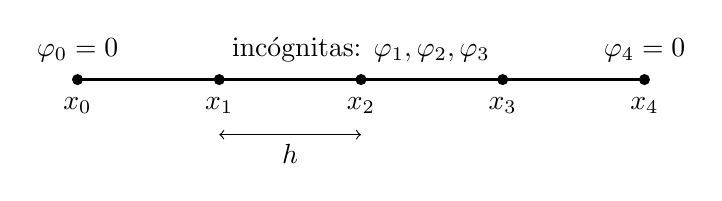
\begin{tikzpicture}[x=1.8cm]
  \draw[thick] (0,0) -- (4,0);
  \foreach \i in {0,...,4} {
    \fill (\i,0) circle (2pt);
    \node[below=3pt] at (\i,0) {$x_{\i}$};
  }
  \node[above=3pt] at (0,0) {$\varphi_0 = 0$};
  \node[above=3pt] at (4,0) {$\varphi_4 = 0$};
  \node[above=3pt] at (2,0) {incógnitas: $\varphi_1, \varphi_2, \varphi_3$};
  \draw[<->] (1,-0.7) -- node[below] {$h$} (2,-0.7);
\end{tikzpicture}
\end{center}
Los valores en $x_0$ y $x_4$ ya se conocen por las condiciones de frontera y quedan solo 3 incognitas

\paso{2}{Colocación de la EDP en $x = x_i$}
\[
  \left.\frac{\partial\varphi}{\partial t}\right|_{x_i}
  = vD \left.\frac{\partial^2\varphi}{\partial x^2}\right|_{x_i} - v\Sigma_a\, \varphi(x_i, t),
  \qquad i = 1, 2, 3 .
\]

\paso{3}{Cambio de la segunda derivada por la segunda diferencia dividida centrada}
Con Taylor alrededor de $x_i$ 
\begin{align*}
  \varphi(x_i + h, t) &= \varphi + h\,\varphi_x + \frac{h^2}{2}\varphi_{xx}
     + \frac{h^3}{6}\varphi_{xxx} + \frac{h^4}{24}\varphi_{xxxx} + \Order{h^5}\\
  \varphi(x_i - h, t) &= \varphi - h\,\varphi_x + \frac{h^2}{2}\varphi_{xx}
     - \frac{h^3}{6}\varphi_{xxx} + \frac{h^4}{24}\varphi_{xxxx} - \Order{h^5}
\end{align*}
Al sumar, los términos de orden impar se cancelan
\begin{align*}
  \varphi(x_i + h, t) &= \varphi + \cancel{h\,\varphi_x} + \frac{h^2}{2}\varphi_{xx}
     + \cancel{\frac{h^3}{6}\varphi_{xxx}} + \frac{h^4}{24}\varphi_{xxxx} + \cdots\\
  \varphi(x_i - h, t) &= \varphi - \cancel{h\,\varphi_x} + \frac{h^2}{2}\varphi_{xx}
     - \cancel{\frac{h^3}{6}\varphi_{xxx}} + \frac{h^4}{24}\varphi_{xxxx} - \cdots
\end{align*}
y los pares se duplican ($\frac{h^2}{2} + \frac{h^2}{2} = h^2$ y
$\frac{h^4}{24} + \frac{h^4}{24} = \frac{h^4}{12}$):
\[
  \varphi(x_{i+1}, t) + \varphi(x_{i-1}, t) = 2\varphi(x_i, t) + h^2\varphi_{xx} + \frac{h^4}{12}\varphi_{xxxx} + \Order{h^6}.
\]
Despejando y dividiendo entre $h^2$ $\left(\frac{h^4}{h^2} = h^2\right)$:
\begin{align*}
  \left.\frac{\partial^2\varphi}{\partial x^2}\right|_{(x_i,t)}
  &= \frac{\varphi(x_{i+1}, t) - 2\varphi(x_i, t) + \varphi(x_{i-1}, t)}{h^2} - \frac{h^2}{12}\varphi_{xxxx} + \Order{h^4}\\
  &= \frac{\varphi(x_{i+1}, t) - 2\varphi(x_i, t) + \varphi(x_{i-1}, t)}{h^2} + \Order{h^2}.
\end{align*}

Simplificación
ahora son aproximaciones
$\varphi_i(t) \approx \varphi(x_i, t)$. Lo introducimos en la EDP:
\[
  \frac{\dd\varphi_i}{\dd t} = vD\,\frac{\varphi_{i+1} - 2\varphi_i + \varphi_{i-1}}{h^2} - v\Sigma_a\, \varphi_i
\]
Se reparte $vD/h^2$ y se agrupan los términos de $\varphi_i$
\[
  \frac{\dd\varphi_i}{\dd t}
  = \frac{vD}{h^2}\, \varphi_{i-1} - \left(\frac{2vD}{h^2} + v\Sigma_a\right) \varphi_i
     + \frac{vD}{h^2}\, \varphi_{i+1}, \qquad i = 1, 2, 3
\]
Con $vD/h^2 = 1$ y $v\Sigma_a = 0$
\[
  \frac{\dd\varphi_i}{\dd t} = \varphi_{i-1} - 2\varphi_i + \varphi_{i+1}
\]
Sustituyendo cada nodo, con $\varphi_0 = \varphi_4 = 0$
\begin{align*}
  i = 1:&\quad \frac{\dd\varphi_1}{\dd t} = \cancelto{0}{\varphi_0} - 2\varphi_1 + \varphi_2 = -2\varphi_1 + \varphi_2\\
  i = 2:&\quad \frac{\dd\varphi_2}{\dd t} = \varphi_1 - 2\varphi_2 + \varphi_3\\
  i = 3:&\quad \frac{\dd\varphi_3}{\dd t} = \varphi_2 - 2\varphi_3 + \cancelto{0}{\varphi_4} = \varphi_2 - 2\varphi_3
\end{align*}
En forma matricial
\[
  \frac{\dd}{\dd t}\begin{pmatrix} \varphi_1\\ \varphi_2\\ \varphi_3 \end{pmatrix}
  = \begin{pmatrix} -2 & 1 & 0\\ 1 & -2 & 1\\ 0 & 1 & -2 \end{pmatrix}
    \begin{pmatrix} \varphi_1\\ \varphi_2\\ \varphi_3 \end{pmatrix}
  = -\underbrace{\begin{pmatrix} 2 & -1 & 0\\ -1 & 2 & -1\\ 0 & -1 & 2 \end{pmatrix}}_{\mat{A}}
    \begin{pmatrix} \varphi_1\\ \varphi_2\\ \varphi_3 \end{pmatrix}
  \quad\Longrightarrow\quad
  \frac{\dd\vect{\varphi}}{\dd t} = -\mat{A}\vect{\varphi} 
\]

\paso{1}{Generación del mallado en tiempo}
\[
  t_n = t_0 + n\,\Delta t, \qquad n = 0, 1, 2, \dots, \qquad
  \vect{\varphi}^{n} \approx \vect{\varphi}(t_n) 
\]

\paso{2}{Colocación del sistema en $t_{n+1/2}$}
Para CN el sistema se coloca en el punto medio $t_{n+1/2} = t_n + \Delta t/2$
\[
  \left.\frac{\dd\vect{\varphi}}{\dd t}\right|_{t_{n+1/2}} = -\mat{A}\,\vect{\varphi}(t_{n+1/2})
\]

\paso{3}{Diferencia centrada y promedio en $t_{n+1/2}$}
Con Taylor alrededor de $t_{n+1/2}$
\begin{align*}
  \vect{\varphi}(t_{n+1}) &= \vect{\varphi} + \frac{\Delta t}{2}\,\vect{\varphi}' + \frac{1}{2}\left(\frac{\Delta t}{2}\right)^2\vect{\varphi}''
     + \frac{1}{6}\left(\frac{\Delta t}{2}\right)^3\vect{\varphi}''' + \cdots
   = \vect{\varphi} + \frac{\Delta t}{2}\,\vect{\varphi}' + \frac{\Delta t^2}{8}\,\vect{\varphi}''
     + \frac{\Delta t^3}{48}\,\vect{\varphi}''' + \cdots\\
  \vect{\varphi}(t_{n}) &= \vect{\varphi} - \frac{\Delta t}{2}\,\vect{\varphi}' + \frac{\Delta t^2}{8}\,\vect{\varphi}''
     - \frac{\Delta t^3}{48}\,\vect{\varphi}''' + \cdots
\end{align*}
Restando se cancelan los términos pares
\begin{align*}
  \vect{\varphi}(t_{n+1}) - \vect{\varphi}(t_n)
  &= \cancel{\vect{\varphi}} - \cancel{\vect{\varphi}} + \frac{\Delta t}{2}\,\vect{\varphi}' + \frac{\Delta t}{2}\,\vect{\varphi}'
     + \cancel{\frac{\Delta t^2}{8}\,\vect{\varphi}''} - \cancel{\frac{\Delta t^2}{8}\,\vect{\varphi}''}
     + \frac{\Delta t^3}{48}\,\vect{\varphi}''' + \frac{\Delta t^3}{48}\,\vect{\varphi}''' + \cdots\\
  &= \Delta t\,\vect{\varphi}' + \frac{\Delta t^3}{24}\,\vect{\varphi}''' + \cdots\\
  \left.\frac{\dd\vect{\varphi}}{\dd t}\right|_{t_{n+1/2}}
  &= \frac{\vect{\varphi}(t_{n+1}) - \vect{\varphi}(t_n)}{\Delta t} - \frac{\Delta t^2}{24}\,\vect{\varphi}''' - \cdots
   = \frac{\vect{\varphi}(t_{n+1}) - \vect{\varphi}(t_n)}{\Delta t} + \Order{\Delta t^2}.
\end{align*}
Sumando  se cancelan los impares
\begin{align*}
  \vect{\varphi}(t_{n+1}) + \vect{\varphi}(t_n)
  &= 2\vect{\varphi} + \cancel{\frac{\Delta t}{2}\,\vect{\varphi}'} - \cancel{\frac{\Delta t}{2}\,\vect{\varphi}'}
     + \frac{\Delta t^2}{8}\,\vect{\varphi}'' + \frac{\Delta t^2}{8}\,\vect{\varphi}''
     + \cancel{\frac{\Delta t^3}{48}\,\vect{\varphi}'''} - \cancel{\frac{\Delta t^3}{48}\,\vect{\varphi}'''} + \cdots\\
  &= 2\vect{\varphi} + \frac{\Delta t^2}{4}\,\vect{\varphi}'' + \cdots\\
  \vect{\varphi}(t_{n+1/2}) &= \frac{\vect{\varphi}(t_{n+1}) + \vect{\varphi}(t_n)}{2} - \frac{\Delta t^2}{8}\,\vect{\varphi}'' - \cdots
   = \frac{\vect{\varphi}(t_{n+1}) + \vect{\varphi}(t_n)}{2} + \Order{\Delta t^2}.
\end{align*}
Se sustituye 
\[
  \frac{\vect{\varphi}^{n+1} - \vect{\varphi}^{n}}{\Delta t} = -\mat{A}\,\frac{\vect{\varphi}^{n+1} + \vect{\varphi}^{n}}{2} .
\]

Parte algebraica
\begin{align*}
  \vect{\varphi}^{n+1} - \vect{\varphi}^{n}
    &= -\frac{\Delta t}{2}\mat{A}\vect{\varphi}^{n+1} - \frac{\Delta t}{2}\mat{A}\vect{\varphi}^{n}
    && \\
  \vect{\varphi}^{n+1} + \frac{\Delta t}{2}\mat{A}\vect{\varphi}^{n+1}
    &= \vect{\varphi}^{n} - \frac{\Delta t}{2}\mat{A}\vect{\varphi}^{n}
    && \\
  \mat{I}\vect{\varphi}^{n+1} + \frac{\Delta t}{2}\mat{A}\vect{\varphi}^{n+1}
    &= \mat{I}\vect{\varphi}^{n} - \frac{\Delta t}{2}\mat{A}\vect{\varphi}^{n}
    && \\
  \left(\mat{I} + \frac{\Delta t}{2}\mat{A}\right)\vect{\varphi}^{n+1}
    &= \left(\mat{I} - \frac{\Delta t}{2}\mat{A}\right)\vect{\varphi}^{n}
    &&
\end{align*}
\resultado{\left(\mat{I} + \tfrac{\Delta t}{2}\mat{A}\right)\vect{\varphi}^{n+1}
	= \left(\mat{I} - \tfrac{\Delta t}{2}\mat{A}\right)\vect{\varphi}^{n}, \qquad n = 0, 1, 2, \dots}

Despejando $\vect{\varphi}^{n+1}$:
\[
\vect{\varphi}^{n+1} = \left(\mat{I} + \frac{\Delta t}{2}\mat{A}\right)^{-1}\left(\mat{I} - \frac{\Delta t}{2}\mat{A}\right)\vect{\varphi}^{n}.
\]
Matrices 
\[
  \frac{\Delta t}{2}\mat{A}
  = \begin{pmatrix}
      \frac{\Delta t}{2}(2) & \frac{\Delta t}{2}(-1) & 0\\[3pt]
      \frac{\Delta t}{2}(-1) & \frac{\Delta t}{2}(2) & \frac{\Delta t}{2}(-1)\\[3pt]
      0 & \frac{\Delta t}{2}(-1) & \frac{\Delta t}{2}(2)
    \end{pmatrix}
  = \begin{pmatrix}
      \Delta t & -\frac{\Delta t}{2} & 0\\[3pt]
      -\frac{\Delta t}{2} & \Delta t & -\frac{\Delta t}{2}\\[3pt]
      0 & -\frac{\Delta t}{2} & \Delta t
    \end{pmatrix},
\]
y sumando y restando con la identidad (solo cambia la diagonal):
\[
  \underbrace{\begin{pmatrix}
      1 + \Delta t & -\frac{\Delta t}{2} & 0\\[3pt]
      -\frac{\Delta t}{2} & 1 + \Delta t & -\frac{\Delta t}{2}\\[3pt]
      0 & -\frac{\Delta t}{2} & 1 + \Delta t
  \end{pmatrix}}_{\mat{I} + \frac{\Delta t}{2}\mat{A}}
  \begin{pmatrix} \varphi_1^{n+1}\\[3pt] \varphi_2^{n+1}\\[3pt] \varphi_3^{n+1} \end{pmatrix}
  =
  \underbrace{\begin{pmatrix}
      1 - \Delta t & \frac{\Delta t}{2} & 0\\[3pt]
      \frac{\Delta t}{2} & 1 - \Delta t & \frac{\Delta t}{2}\\[3pt]
      0 & \frac{\Delta t}{2} & 1 - \Delta t
  \end{pmatrix}}_{\mat{I} - \frac{\Delta t}{2}\mat{A}}
  \begin{pmatrix} \varphi_1^{n}\\[3pt] \varphi_2^{n}\\[3pt] \varphi_3^{n} \end{pmatrix}.
\]
Haciendo los productos renglon por renglon queda la forma nodal:
\begin{align*}
  i = 1:&\quad (1 + \Delta t)\,\varphi_1^{n+1} - \tfrac{\Delta t}{2}\,\varphi_2^{n+1}
          = (1 - \Delta t)\,\varphi_1^{n} + \tfrac{\Delta t}{2}\,\varphi_2^{n}\\
  i = 2:&\quad -\tfrac{\Delta t}{2}\,\varphi_1^{n+1} + (1 + \Delta t)\,\varphi_2^{n+1} - \tfrac{\Delta t}{2}\,\varphi_3^{n+1}
          = \tfrac{\Delta t}{2}\,\varphi_1^{n} + (1 - \Delta t)\,\varphi_2^{n} + \tfrac{\Delta t}{2}\,\varphi_3^{n}\\
  i = 3:&\quad -\tfrac{\Delta t}{2}\,\varphi_2^{n+1} + (1 + \Delta t)\,\varphi_3^{n+1}
          = \tfrac{\Delta t}{2}\,\varphi_2^{n} + (1 - \Delta t)\,\varphi_3^{n}
\end{align*}


\inciso{b}{por factorización triple}


\paso{1}{Armar el sistema}
Con $\Delta t = \frac12$:
\[
  \frac{\Delta t}{2} = \frac{1/2}{2} = \frac14, \qquad
  1 + \Delta t = 1 + \frac12 = \frac32, \qquad
  1 - \Delta t = 1 - \frac12 = \frac12 .
\]
\[
  \mat{B} = \mat{I} + \frac14\mat{A} =
  \begin{pmatrix} \frac32 & -\frac14 & 0\\[3pt] -\frac14 & \frac32 & -\frac14\\[3pt] 0 & -\frac14 & \frac32 \end{pmatrix},
  \qquad
  \mat{C} = \mat{I} - \frac14\mat{A} =
  \begin{pmatrix} \frac12 & \frac14 & 0\\[3pt] \frac14 & \frac12 & \frac14\\[3pt] 0 & \frac14 & \frac12 \end{pmatrix}.
\]
Lado derecho con $\vect{\varphi}^0 = (0, 1, 0)^T$, rengln por renglon
\[
  \vect{b} = \mat{C}\vect{\varphi}^0 =
  \begin{pmatrix}
    \frac12(0) + \frac14(1) + 0(0)\\[3pt]
    \frac14(0) + \frac12(1) + \frac14(0)\\[3pt]
    0(0) + \frac14(1) + \frac12(0)
  \end{pmatrix}
  = \begin{pmatrix} \frac14\\[3pt] \frac12\\[3pt] \frac14 \end{pmatrix}.
\]
se multiplica todo el sistema por $4$

\[
4\cdot\frac32 = 6, \qquad 4\left(-\frac14\right) = -1, \qquad
4\cdot\frac14 = 1, \qquad 4\cdot\frac12 = 2,
\]
\[
4\mat{B}\begin{pmatrix} \varphi_1^1\\ \varphi_2^1\\ \varphi_3^1 \end{pmatrix} = 4\vect{b}
\qquad\text{o sea}\qquad
\begin{pmatrix} 6 & -1 & 0\\ -1 & 6 & -1\\ 0 & -1 & 6 \end{pmatrix}
\begin{pmatrix} \varphi_1^1\\ \varphi_2^1\\ \varphi_3^1 \end{pmatrix}
= \begin{pmatrix} 1\\ 2\\ 1 \end{pmatrix} .
\]
Primero $\mat{D}\mat{L}^T$ (cada renglón de $\mat{L}^T$ se multiplica por su $d_{ii}$):
\[
  \mat{D}\mat{L}^T = \begin{pmatrix} d_{11} & d_{11}l_{21} & d_{11}l_{31}\\ 0 & d_{22} & d_{22}l_{32}\\ 0 & 0 & d_{33} \end{pmatrix},
\]
y luego $\mat{L}(\mat{D}\mat{L}^T)$:
\[
  \mat{L}\mat{D}\mat{L}^T =
  \begin{pmatrix}
    d_{11} & d_{11}l_{21} & d_{11}l_{31}\\
    l_{21}d_{11} & l_{21}^2 d_{11} + d_{22} & l_{21}l_{31}d_{11} + l_{32}d_{22}\\
    l_{31}d_{11} & l_{31}l_{21}d_{11} + l_{32}d_{22} & l_{31}^2 d_{11} + l_{32}^2 d_{22} + d_{33}
  \end{pmatrix}.
\]

\begin{align*}
  (1,1):&\quad d_{11} = 6\\
  (1,2):&\quad d_{11}l_{21} = -1 \;\Longrightarrow\; 6\,l_{21} = -1 \;\Longrightarrow\; l_{21} = -\frac16\\
  (1,3):&\quad d_{11}l_{31} = 0 \;\Longrightarrow\; 6\,l_{31} = 0 \;\Longrightarrow\; l_{31} = 0\\
  (2,2):&\quad l_{21}^2 d_{11} + d_{22} = 6 \;\Longrightarrow\;
           \left(-\frac16\right)^2(6) + d_{22} = 6 \;\Longrightarrow\;
           \frac16 + d_{22} = 6 \;\Longrightarrow\; d_{22} = \frac{36 - 1}{6} = \frac{35}{6}\\
  (2,3):&\quad l_{21}\cancelto{0}{l_{31}}\,d_{11} + l_{32}d_{22} = -1 \;\Longrightarrow\;
           l_{32}\left(\frac{35}{6}\right) = -1 \;\Longrightarrow\; l_{32} = -\frac{6}{35}\\
  (3,3):&\quad \cancelto{0}{l_{31}^2}\,d_{11} + l_{32}^2 d_{22} + d_{33} = 6 \;\Longrightarrow\;
           \left(-\frac{6}{35}\right)^2\left(\frac{35}{6}\right) + d_{33} = 6
\end{align*}
\[
  \left(-\frac{6}{35}\right)^2\left(\frac{35}{6}\right)
  = \frac{6\cdot\cancel{6}}{35\cdot\cancel{35}}\cdot\frac{\cancel{35}}{\cancel{6}}
  = \frac{6}{35}
  \quad\Longrightarrow\quad
  d_{33} = 6 - \frac{6}{35} = \frac{210 - 6}{35} = \frac{204}{35}.
\]

resultado
\resultado{\tilde{\mat{B}} =
  \begin{pmatrix} 1 & 0 & 0\\ -\frac16 & 1 & 0\\ 0 & -\frac{6}{35} & 1 \end{pmatrix}
  \begin{pmatrix} 6 & 0 & 0\\ 0 & \frac{35}{6} & 0\\ 0 & 0 & \frac{204}{35} \end{pmatrix}
  \begin{pmatrix} 1 & -\frac16 & 0\\ 0 & 1 & -\frac{6}{35}\\ 0 & 0 & 1 \end{pmatrix}}

Los tres pivotes $6, \frac{35}{6}, \frac{204}{35}$ son positivos como se esperaba de una matriz simétrica definida positiva.

\textbf{(i) Sustitución hacia adelante} $\mat{L}\vect{z} = 4\vect{b}$:
\[
  \begin{pmatrix} 1 & 0 & 0\\ -\frac16 & 1 & 0\\ 0 & -\frac{6}{35} & 1 \end{pmatrix}
  \begin{pmatrix} z_1\\ z_2\\ z_3 \end{pmatrix} = \begin{pmatrix} 1\\ 2\\ 1 \end{pmatrix}
\]
\begin{align*}
  z_1 &= 1\\
  -\frac16 z_1 + z_2 = 2 \;\Longrightarrow\; z_2 &= 2 + \frac16(1) = \frac{12 + 1}{6} = \frac{13}{6}\\
  -\frac{6}{35} z_2 + z_3 = 1 \;\Longrightarrow\; z_3 &= 1 + \frac{\cancel{6}}{35}\cdot\frac{13}{\cancel{6}}
     = 1 + \frac{13}{35} = \frac{35 + 13}{35} = \frac{48}{35}
\end{align*}

\textbf{(ii) Escalamiento} $\mat{D}\vect{y} = \vect{z}$
\begin{align*}
  y_1 &= \frac{z_1}{d_{11}} = \frac{1}{6}\\
  y_2 &= \frac{z_2}{d_{22}} = \frac{13/6}{35/6} = \frac{13}{{6}}\cdot\frac{{6}}{35} = \frac{13}{35}\\
  y_3 &= \frac{z_3}{d_{33}} = \frac{48/35}{204/35} = \frac{48}{{35}}\cdot\frac{{35}}{204}
       = \frac{48}{204} = \frac{48 \div 12}{204 \div 12} = \frac{4}{17}
\end{align*}

\textbf{(iii) Sustitución hacia atrás,} $\mat{L}^T\vect{\varphi}^1 = \vect{y}$:
\[
  \begin{pmatrix} 1 & -\frac16 & 0\\ 0 & 1 & -\frac{6}{35}\\ 0 & 0 & 1 \end{pmatrix}
  \begin{pmatrix} \varphi_1^1\\ \varphi_2^1\\ \varphi_3^1 \end{pmatrix} = \begin{pmatrix} \frac16\\[3pt] \frac{13}{35}\\[3pt] \frac{4}{17} \end{pmatrix}
\]
\begin{align*}
  \varphi_3^1 &= \frac{4}{17}\\
  \varphi_2^1 - \frac{6}{35}\varphi_3^1 = \frac{13}{35} \;\Longrightarrow\; \varphi_2^1
    &= \frac{13}{35} + \frac{6}{35}\cdot\frac{4}{17}
     = \frac{13\cdot 17}{35\cdot 17} + \frac{24}{595}
     = \frac{221 + 24}{595} = \frac{245}{595} = \frac{245 \div 35}{595 \div 35} = \frac{7}{17}\\
  \varphi_1^1 - \frac16 \varphi_2^1 = \frac16 \;\Longrightarrow\; \varphi_1^1
    &= \frac16 + \frac16\cdot\frac{7}{17} = \frac16\left(1 + \frac{7}{17}\right)
     = \frac{1}{6}\cdot\frac{24}{17} = \frac{24}{102} = \frac{4}{17}
\end{align*}
\resultado{\vect{\varphi}^1 = \left(\frac{4}{17},\; \frac{7}{17},\; \frac{4}{17}\right)^T}


% =====================================================================
\inciso{c}{Factor de amplificación de cada modo}
% =====================================================================

\paso{1}{Vectores propios de $\mat{A}$}
Se llaman $\lambda_1 = 2 - \sqrt2$, $\lambda_2 = 2$, $\lambda_3 = 2 + \sqrt2$ y $\vect{w}_j$ al vector propio de $\lambda_j$,
o sea $\mat{A}\vect{w}_j = \lambda_j\vect{w}_j$. Se resuelve $(\mat{A} - \lambda_j\mat{I})\vect{w}_j = \vect{0}$.

Para $\lambda_1 = 2 - \sqrt2$:
\[
\mat{A} - \lambda_1\mat{I} =
\begin{pmatrix} \sqrt2 & -1 & 0\\ -1 & \sqrt2 & -1\\ 0 & -1 & \sqrt2 \end{pmatrix}
\]
\begin{align*}
	\text{renglón 1:}&\quad \sqrt2\,w_1 - w_2 = 0 \;\Longrightarrow\; w_2 = \sqrt2\,w_1\\
	\text{renglón 3:}&\quad -w_2 + \sqrt2\,w_3 = 0 \;\Longrightarrow\; w_3 = \frac{w_2}{\sqrt2} = \frac{\sqrt2\,w_1}{\sqrt2} = w_1\\
	\text{renglón 2:}&\quad -w_1 + \sqrt2\,(\sqrt2\,w_1) - w_1 = -w_1 + 2w_1 - w_1 = 0 \quad (\text{se cumple})
\end{align*}
Con $w_1 = 1$: $\vect{w}_1 = (1, \sqrt2, 1)^T$.

Para $\lambda_2 = 2$:
\[
\mat{A} - \lambda_2\mat{I} =
\begin{pmatrix} 0 & -1 & 0\\ -1 & 0 & -1\\ 0 & -1 & 0 \end{pmatrix}
\]
\begin{align*}
	\text{renglón 1:}&\quad -w_2 = 0 \;\Longrightarrow\; w_2 = 0\\
	\text{renglón 2:}&\quad -w_1 - w_3 = 0 \;\Longrightarrow\; w_3 = -w_1\\
	\text{renglón 3:}&\quad -w_2 = 0 \quad (\text{se cumple})
\end{align*}
Con $w_1 = 1$: $\vect{w}_2 = (1, 0, -1)^T$.

Para $\lambda_3 = 2 + \sqrt2$:
\[
\mat{A} - \lambda_3\mat{I} =
\begin{pmatrix} -\sqrt2 & -1 & 0\\ -1 & -\sqrt2 & -1\\ 0 & -1 & -\sqrt2 \end{pmatrix}
\]
\begin{align*}
	\text{renglón 1:}&\quad -\sqrt2\,w_1 - w_2 = 0 \;\Longrightarrow\; w_2 = -\sqrt2\,w_1\\
	\text{renglón 3:}&\quad -w_2 - \sqrt2\,w_3 = 0 \;\Longrightarrow\; w_3 = -\frac{w_2}{\sqrt2} = \frac{\sqrt2\,w_1}{\sqrt2} = w_1\\
	\text{renglón 2:}&\quad -w_1 - \sqrt2\,(-\sqrt2\,w_1) - w_1 = -w_1 + 2w_1 - w_1 = 0 \quad (\text{se cumple})
\end{align*}
Con $w_1 = 1$: $\vect{w}_3 = (1, -\sqrt2, 1)^T$.

\resultado{\vect{w}_1 = \begin{pmatrix} 1\\ \sqrt2\\ 1 \end{pmatrix},\quad
	\vect{w}_2 = \begin{pmatrix} 1\\ 0\\ -1 \end{pmatrix},\quad
	\vect{w}_3 = \begin{pmatrix} 1\\ -\sqrt2\\ 1 \end{pmatrix}}



\inciso{d}{Euler explícito contra CN}

